%%%%%%%%%%%%%%%%%%%%%%%%%%%%%%%%%%%%%%%%%
% University/School Laboratory Report
% LaTeX Template
% Version 3.1 (25/3/14)
%
% This template has been downloaded from:
% http://www.LaTeXTemplates.com
%
% Original author:
% Linux and Unix Users Group at Virginia Tech Wiki 
% (https://vtluug.org/wiki/Example_LaTeX_chem_lab_report)
%
% License:
% CC BY-NC-SA 3.0 (http://creativecommons.org/licenses/by-nc-sa/3.0/)
%
%%%%%%%%%%%%%%%%%%%%%%%%%%%%%%%%%%%%%%%%%

%----------------------------------------------------------------------------------------
%	PACKAGES AND DOCUMENT CONFIGURATIONS
%----------------------------------------------------------------------------------------

\documentclass{article}

%\usepackage[version=3]{mhchem} % Package for chemical equation typesetting
\usepackage{siunitx} % Provides the \SI{}{} and \si{} command for typesetting SI units
\usepackage{graphicx} % Required for the inclusion of images
\usepackage{natbib} % Required to change bibliography style to APA
\usepackage{amsmath} % Required for some math elements 
\usepackage[utf8]{inputenc} % Required for special characters processing
%
\usepackage{fullpage} % changes the margin
\setlength\parindent{0pt} % Removes all indentation from paragraphs

\renewcommand{\labelenumi}{\alph{enumi}.} % Make numbering in the enumerate environment by letter rather than number (e.g. section 6)

\usepackage{times} % Uncomment to use the Times New Roman font

%----------------------------------------------------------------------------------------
%	DOCUMENT INFORMATION
%----------------------------------------------------------------------------------------

\title{\textbf{Air Density and Humidity} \\ Meteorology
  \& Climatology} % Title

\author{Environmental Science Degree} % Author name

\date{\today} % Date for the report

\begin{document}

\maketitle % Insert the title, author and date

\begin{center}
\begin{tabular}{l r}
Date Performed: & \underline{\hspace{3cm}}  \\ % Date the experiment was performed
Partners: & \underline{\hspace{6cm}} \\ % Partner names
& \underline{\hspace{6cm}} \\
& \underline{\hspace{6cm}} \\
Instructor: & Prof.~F.~Pérez-Bernal % Instructor/supervisor
\end{tabular}
\end{center}

% If you wish to include an abstract, uncomment the lines below
\begin{abstract}
  In this lab session the dewpoint temperature ($\tau$), relative humidity ($h$),
  and water vapor pressure ($e$) at the laboratory are measured.
  Using these data the dry air density at standard conditions of
  pressure ($p = \SI{1}{atm}$) and temperature ($T= \SI{273.15}{K}$) is
  computed.
\end{abstract}

%----------------------------------------------------------------------------------------
%	SECTION 1
%----------------------------------------------------------------------------------------
\section{Introduction}
According to Dalton Law, the air pressure in the lab is the sum of
dry air pressure ($p_d$) plus the \textbf{partial pressure of water vapor}
($e$). Therefore $p = e + p_d$ with $p_d>>e$.

The partial water vapor pressure, also called vapor pressure and vapor
tension, and denoted by $e$ has a maximum value that depends on the
temperature which is denoted with the uppercase letter, $E = E(T)$.

\textbf{Relative humidity} of an air parcel is defined as $h = 100\frac{e}{E}$,
therefore $0\le h\le 100$, and is dependent on the water vapor content of
the air (through $e$) and of temperature (through $E$).

\textbf{Dewpoint  temperature} ($\tau$)  of an  air  parcel is  defined as  the
temperature to  which a  given air parcel  must be cooled \textit{ at constant
pressure and constant  water vapor content} in order  for saturation to
occur.

In order to measure water vapor contents of the air the device used is
a \textbf{hygrometer} and among the different types of hygrometer a
psychrometer, a sling psychrometer, and a simple chilled mirror
dewpoint hygrometer.

The knowledge of $e$, $h$, or $\tau$ makes possible to assess the mass
of water vapor in a sample of air and, combining these results with
$T$ and $p$ measurements after some manipulations with the state
equation of ideal gases the density of dry air at standard conditions
can be obtained.
 


\section{Objectives}

The objective of this lab session is to \textit{measure the lab air
  humidity} using three different types of hygrometers and use these
measurements to compute \textit{dry air density at standard
  conditions}.

As a bonus, a second objective of the lab session is to appropriately identify the
\textit{possible sources of errors and your results possible uncertainties}. 


\section{Theoretical Basis and Lab Procedures}

\subsection{Mirror dewpoint hygrometer $e$ measurement}

The first measurements performed are done with the chilled mirror
dewpoint hygrometer (see the schematic view in Fig.\
\ref{fig_mirrordew}). A small quantity of \textit{N-pentane} is
introduced into the metalic hygrometer cyllinder, such that the tip of
the digital thermometer rests very close to the surface of the
\textit{N-pentane} or just below it.

\vspace{0.2cm}
IMPORTANT NOTE: \textbf{Please, note that N-pentane is a clear colorless liquid with a
  petroleum-like odor. It is highly flammable and its vapors may cause
  drowsiness or dizziness. It may be fatal if once swallowed enters
  airways. Handle with care.
}
\vspace{0.2cm}

\begin{figure}[h]
\begin{center}
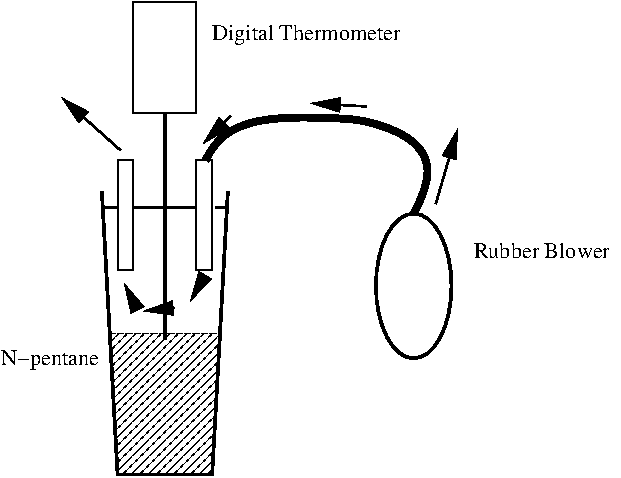
\includegraphics[width=0.5\textwidth]{Figs/hygro.png} % Include the image placeholder.png
\caption{Scheme of the chilled mirror
dewpoint hygrometer.}\label{fig_mirrordew}
\end{center}
\end{figure}


The chilled mirror dewpoint hygrometer makes possible a direct
measurement of the dew point temperature. The forced circulation of
air over the \textit{N-pentane} surface making use of the rubber
blower produces a decrease of temperature due to the evaporation of
the highly volatile substance. This lowers the temperature on the
metallic tube and once the dewpoint temperature is reached
condensation starts and minute water drops can be seen on the
metallic surface. Record the dew point temperature $\tau$. This
procedure should be repeated four times and \textit{the mean value
of the four measured dewpoint temperatures is the air dewpoint temperature and the standard deviation of the values its error}. 

\vspace{0.2cm}
IMPORTANT NOTE 2:  \textbf{You should stop blowing air at the first signals
  of condensation (can be quite complicated to appreciate), do not
  wait till water is clearly visible as once reached this point then
  the temperature is for sure much lower than the actual dew point.}

\vspace{0.2cm}
One of the main objectives of this lab session is that you understand
why the saturation vapor tension of a mass of air at the dewpoint
temperature is equal to the vapor tension of the air mass
\begin{equation}
e = E(\tau)~.
\end{equation}
Thus, you can find the value of the vapor tension for the lab air as $e = E(\tau)$
from the data in Tab.\ 1 performing a linear interpolation
if necessary.

Once $e$ is known, the laboratory air temperature ($T_{lab}$) can be
measured and $E(T_{lab})$ can be obtained from  Tab.\ 1, and the relative humidity of the air can be computed as 

\begin{equation}
h = 100\frac{e}{E} = 100 \frac{E(\tau)}{E(T_{lab})}~.
\label{heq}
\end{equation}

\subsection{Measuring relative humidity with psychrometers}
A dry and wet-bulb pyschrometer is used and the dry bulb temperature
and the wet-bulb depression records are used to obtain the air
relative humidity $h$ making use of the associated \textit{psychrometric
  table}. Making use of the $E(T_{lab})$ value from the previous
subsection the value of $e$ for the lab air can be obtained from Eq.\
\eqref{heq}.

The same procedure is performed for the sling psychrometer with its \textit{psychrometric
  table}.

\subsection{Dry air density at standard conditions}

Normalized dry air density is characterized by the following parameters
\begin{itemize}
\item
Vapor tension: $e = \SI{0}{hPa}$.
\item
Air Temperature: $T_0 = \SI{273.15}{K}$.
\item
Air pressure: $p_0 = \SI{1013.25}{hPa}$.
\end{itemize}

The first step consists of measuring the density of the lab air making
use of a glass sphere with two valves, a precision balance, and a
vacuum pump. The mass of the glass sphere full of air, $m_1$, is
measured. Afterwards, the air is extracted with the pump and the mass
of the sphere without air is measured, $m_0$. The mass of air in the
sphere is $m_{air} = m_1 - m_0$. 

In order to calculate $V_{air}$, the volume
occupied by the gas, \textit{taking care of not breaking the vacuum
  into the sphere}, we proceed to fill it with the water provided in a
beaker and we measure the water temperature $T_w$. We measure the
weight of the sphere with water inside, $m_2$, and the mass of water
into the sphere is $m_{water} = m_2 - m_0$. From Tab.\ 2 we can compute the water density at $T_w$
temperature and thus the density of the air is

{\Large
\begin{equation} 
\bar\rho = \frac{m_{air}}{V_{air}} =\frac{m_1-m_0}{m_2-m_0} \rho_{w}(T_w)~.
\end{equation}
}

It can be demonstrated that the density of humid air $\bar\rho$ can be expressed as a function of dry air density ($\rho_d$), vapor tension ($e$) and dry air pressure ($p_d$) as follows
\begin{equation} 
\bar \rho  = \rho_d \left( 1  +  \epsilon \frac{e}{p_d} \right)~,
\label{eq_barrho}
\end{equation}
\noindent where $\epsilon$ is the ration of water and dry air molecular masses: $\epsilon = M_w/M_d = 0.622$.

We continue measuring the laboratory air pressure and temperature, $p$ and $T$ and the dry air density at this conditions, $\rho_d$ is related to the dry air density value at standard conditions $rho_0$ with the formula
\begin{equation} 
\rho_0 = \rho_d  \frac{T}{T_0}  \frac{p_0}{p_d}~.
\end{equation} 
Taking Eq.\ \eqref{eq_barrho} into account we obtain
{\Large
\begin{equation} 
\rho_0 = \bar\rho \, \frac{T}{T_0} \, \frac{p_0}{p} \,
\left[
1 - (1-\epsilon) \frac{e}{p}
\right]^{-1}~.
\end{equation}
}

The  standard density  $\rho_0$ is  then  computed making  use of  the
different values  of the vapor tension  obtained in the first  part of
the  lab session  and the  results obtained  as well  as their  errors
should be discussed.

\section{Experimental Data}

\subsection{Mirror dewpoint hygrometer measurements}

\begin{tabular}{|c|c|c|c|c|c|}
\hline
$\tau_1$&$\tau_2$&$\tau_3$&$\tau_4$&$\bar \tau$ &$\sigma_\tau$\\
\hline
~\hspace{2.25cm}~&~\hspace{2.25cm}~&~\hspace{2.25cm}~&~\hspace{2.25cm}~&~\hspace{2.5cm}~&~\hspace{2.5cm}~\\
\hline
\end{tabular}

\vspace{5mm}

Dewpoint Temperature: $\tau \pm E_\tau = $ \underline{\hspace{4cm}}

\vspace{5mm}

Air Temperature: $T \pm E_T = $ \underline{\hspace{4cm}}


\subsection{Wall psychrometer measurements}

Dry bulb temperature: $T_{\mbox{dry}}=$ \underline{\hspace{3cm}}  \hspace{1cm}
Wet bulb temperature: $T_{\mbox{wet}}=$ \underline{\hspace{3cm}}

\vspace{5mm}

Relative humidity\footnote{Consider that the wall psychrometer relative humidity values have a 5\% relative error.}: $h \pm E_h= $\underline{\hspace{3cm}}


\subsection{Sling psychrometer measurements}

Dry bulb temperature: $T_{\mbox{dry}}=$ \underline{\hspace{3cm}}  \hspace{1cm}
Wet bulb temperature: $T_{\mbox{wet}}=$ \underline{\hspace{3cm}}

\vspace{5mm}

Relative humidity\footnote{Consider that the wall psychrometer relative humidity values have a 3\% relative error.}: $h \pm E_h = $\underline{\hspace{3cm}}


\subsection{Standard air density measurements}


\begin{tabular}{|c|c|c|c|}
\hline
$m_0$&$m_1$&$m_2$&$T_w$\\
\hline
~\hspace{2.5cm}~&~\hspace{2.5cm}~&~\hspace{2.5cm}~&~\hspace{2.5cm}~\\
\hline
\end{tabular}

\vspace{5mm}

Water density\footnote{You can consider an error equal to half of the interval of density values in the table for the considered temperature.}: $\rho_{w} ( T_{w} )\pm E_{\rho_w}=$
\underline{\hspace{2.5cm}}


\vspace{5mm}
Atmospheric pressure: $p =$ \underline{\hspace{4cm}} \hspace{2cm} 


\newpage
\section{Results and Conclusions}

\subsection{Mirror dewpoint hygrometer results}

Vapor tension: $e = E (\tau) = $ \underline{\hspace{4cm}}

\vspace{5mm}

Saturation vapor tension $E = E (T) =$ \underline{\hspace{4cm}}

\vspace{5mm}

Relative Humidity: $h =100\frac{e}{E} = 100\frac{E (\tau)}{E(T)} = $ \underline{\hspace{4cm}}
\subsection{Wall psychrometer results}

Vapor pressure: $e \pm E_e = $
\underline{\hspace{4cm}}

\subsection{Sling psychrometer results}

Vapor pressure: $e \pm E_e = $
\underline{\hspace{4cm}}
\subsection{Standard air density measurements}

Air density: $\overline{\rho} \pm E_{\bar \rho} = $ \underline{\hspace{4cm}}
 
\vspace{5mm}
Standard air density (hygrometer): ~$\rho_0 =$
\underline{\hspace{4cm}}
\vspace{5mm}

Standard air density (psychrometer): ~$\rho_0 =$
\underline{\hspace{4cm}}

\vspace{5mm}

Standard air density (sling psychrometer): ~$\rho_0 =$
\underline{\hspace{4cm}}

\nocite{*}
\newpage
\appendix
\section{Data Tables}


\begin{center}
\begin{tabular}{|c|c||c|c|} \hline
T ($^{\circ}$C)  &  $E$ (mb)  & T ($^{\circ}$C)  & $E$ (mb)  \\
\hline
0  &  6.11  &  17  &  19.37  \\
\hline
1  &  6.56  &  18  &  20.62  \\
\hline
2  &  7.05  &  19  &  21.96  \\
\hline
3  &  7.57  &  20  &  23.37  \\
\hline
4  &  8.13  &  21  &  24.86  \\
\hline
5  &  8.72  &  22  &  26.42  \\
\hline
6  &  9.35  &  23  &  28.09  \\
\hline
7  &  10.05  &  24  &  29.84  \\
\hline
8  &  10.72  &  25  &  31.68  \\
\hline
9  &  11.48  &  26  &  33.61  \\
\hline
10  &  12.27  &  27  &  35.65  \\
\hline
11  &  13.21  &  28  &  37.80  \\
\hline
12  &  14.01  &  29  &  40.05  \\
\hline
13  &  14.97  &  30  &  42.42  \\
\hline
14  &  15.97  &  31  &  44.93  \\
\hline
15  &  17.04  &  32  &  47.56  \\
\hline
16  &  18.17  &  33  &  50.30  \\
\hline
\end{tabular}

Table 1: Water vapor saturation tension $E$ as a function of temperature.
\end{center}

\vspace{0.5cm}
\begin{center}
\begin{tabular}{|c|c||c|c|} \hline
T ($^{\circ}$C)  &  $\rho$ (g/cm$^{3}$) & T ($^{\circ}$C) & $\rho$
(g/cm$^{3}$) \\
\hline
0  &  0.999841  &  16  &  0.998943 \\
\hline
1  &  0.999900  &  17  &  0.998775  \\
\hline
2  &  0.999941  &  18  &  0.998596  \\
\hline
3  &  0.999965  &  19  &  0.998406  \\
\hline
4  &  0.999973  &  20  &  0.998205  \\
\hline
5  &  0.999965  &  21  &  0.997994  \\
\hline
6  &  0.999941  &  22  &  0.997772  \\
\hline
7  &  0.999902  &  23  &  0.997540  \\
\hline
8  &  0.999849  &  24  &  0.997299  \\
\hline
9  &  0.999782  &  25  &  0.997047  \\
\hline
10  &  0.999701  &  26  &  0.996785  \\
\hline
11  &  0.999606  &  27  &  0.996515  \\
\hline
12  &  0.999498  &  28  &  0.996235  \\
\hline
13  &  0.999377  &  29  &  0.995946  \\
\hline
14  &  0.999244  &  30  &  0.995649  \\
\hline
15  &  0.999099  &  &  \\
\hline
\end{tabular}

Table 2: Distilled water density as a function of temperature.
\end{center}

%----------------------------------------------------------------------------------------

\bibliographystyle{apalike}

\bibliography{sample}

%----------------------------------------------------------------------------------------


\end{document}